\documentclass[conference, 11pt]{IEEEtran}
\IEEEoverridecommandlockouts
% The preceding line is only needed to identify funding in the first footnote. If that is unneeded, please comment it out.
\usepackage{cite}
\usepackage{amsmath,amssymb,amsfonts}
\usepackage{algorithmic}
\usepackage{graphicx}
\usepackage{textcomp}
\usepackage{xcolor}
\usepackage{wrapfig}
\usepackage{subcaption}
\def\BibTeX{{\rm B\kern-.05em{\sc i\kern-.025em b}\kern-.08em
    T\kern-.1667em\lower.7ex\hbox{E}\kern-.125emX}}
\begin{document}

\title{Credit Score Classification\\
{\footnotesize GitHub repository: https://github.com/Jacob-Tuttle/ECS171-Project/tree/main}
}

\author{
\IEEEauthorblockN{1\textsuperscript{st} Kyle Jow}
\and
\IEEEauthorblockN{2\textsuperscript{nd} Kyle Pickle}
\and
\IEEEauthorblockN{3\textsuperscript{rd} Jimmy Nguyen}
\and
\IEEEauthorblockN{4\textsuperscript{th} Jacob Tuttle}
\and
\IEEEauthorblockN{5\textsuperscript{th} Kris Wong}

}

\maketitle

% \begin{abstract}
% This document is a model and instructions for \LaTeX.
% This and the IEEEtran.cls file define the components of your paper [title, text, heads, etc.]. *CRITICAL: Do Not Use Symbols, Special Characters, Footnotes, 
% or Math in Paper Title or Abstract.
% \end{abstract}

% \begin{IEEEkeywords}
% component, formatting, style, styling, insert
% \end{IEEEkeywords}

\section{Introduction}
A common problem in the finance and banking industry is assessing the risk involved with lending money to clients.
To better assess a borrower's creditworthiness, lenders formulate and assign “credit scores” to their clients, based on preconceived data 
like income, spending, and credit history.
This score can then be used by a bank as an indicator of whether a client will default or otherwise miss a payment on a given loan.
The rise of cloud-based computing in the 21st century has made it more advantageous and easier than ever for banks to share a
standardized database of credit scores and financial information on their clients.
As a result, credit scoring is being used more and more frequently to determine “worthiness” for almost anything -- qualifying for
mortgages, insurance, and even more nuanced decisions like cell phone plans and determining your employability.
\vspace{5mm}\newline
With this increase in credit scoring has come an increased interest in financial literacy among clients as to how to understand and improve
one's score.
As such, credit standards like FICO and VantageScore have begun giving their clients a way to view an estimation of their credit score, often
provided through the bank and credit card services that utilize them.
These credit score estimates are predicted in a way that is simple for the client to understand, often broken down into categories like
“poor,” “standard,” and “good” and presented alongside graphs displaying factors like age bracket and income to put them into perspective.
This demand for straightforward and transparent credit scoring by governments and clients alike has interestingly compelled banks to
consider less intricate or “black box” machine learning models, creating a delicate balance between accuracy and simplicity.
\vspace{5mm}\newline
credit scoring has always been a common, concrete example of machine learning, as -- in the world of economics -- even the tiniest increase
in accuracy can save billions of dollars in the long-run.
As a result, researchers have utilized a variety of machine learning algorithms to better predict credit scores and risk.
Nearly all client data is now digitized by banks, and with numerous complex variables that drive one's score, credit score prediction
through machine learning is an ideal way to not only predict creditworthiness but constantly tune the equations and hyperparameters used
to determine it in the midst of a fluctuating, real-world economy.

\section{Literature review}
Economists and researchers alike have utilized a variety of machine learning algorithms to better predict credit scores and investment risk.
Some common implementations include decision trees, logistic regression, and Support Vector Machines (SVM).
\vspace{5mm}\newline
% https://www.sciencedirect.com/science/article/pii/S1568494620302039
With the history of credit scoring tracing its roots back to the 1950s, bank decisions were initially guided by the
5 C's approach -- Character, Capital, Collateral, Capacity, and Condition -- relying on subjective, physically-recorded information it its
assessments.
While we could now consider this approach a decision-tree model, Dastile et al. describe how the financial industry's regulatory need for
transparency in lending decisions has led to the prevalence of logistic regression models, known for their simplicity and interpretability.
While sophisticated, higher-accuracy machine learning models have arisen over time, their opacity continues to raise concerns.
In response, Dastile et al. go on to note several key machine learning techniques between 2010 and 2018 that have created a guided
framework of credit scoring, combining both accuracy and transparency in lending decisions [1].
\vspace{5mm}\newline
% https://www.sciencedirect.com/science/article/pii/S0377221721005695#sec0012
One modern approach to credit scoring comes from Dumitrescu et. al., who use a particular model called Penalised Logistic Tree Regression
(PLTR) for credit score classification with an improved logistic regression model that has non-linear decision tree effects [2].
It is able to predict credit score more accurately than the benchmark logistic regression commonly used in the industry, and on a level
that is comparable to more accurate random forest models.
This is because it is able to capture recursive, multi-variable traits in the data unnoticed by a typical logistic regression.
Dumitrescu et. al. use multiple datasets to test the robustness of the model and argue that PLTR preserves the needed transparency and
interpretability that come with logistic regression.

\section{Dataset description and exploratory data analysis}
The dataset contains 27 features. The features we will be focusing on in order
to classify a person's credit score, which is categorical, into either ``good", ``standard", or ``poor" credit
will be features that had the most correlation with credit score according to the heat map
generated from this data and features used in real-life credit score assessing. Although the Credit\_Utilization\_Ratio attribute has little 
correlation to credit score, this feature is used to assess credit in real life, so we kept it. (Figure 1).
\begin{figure}[h]
    \begin{center}
    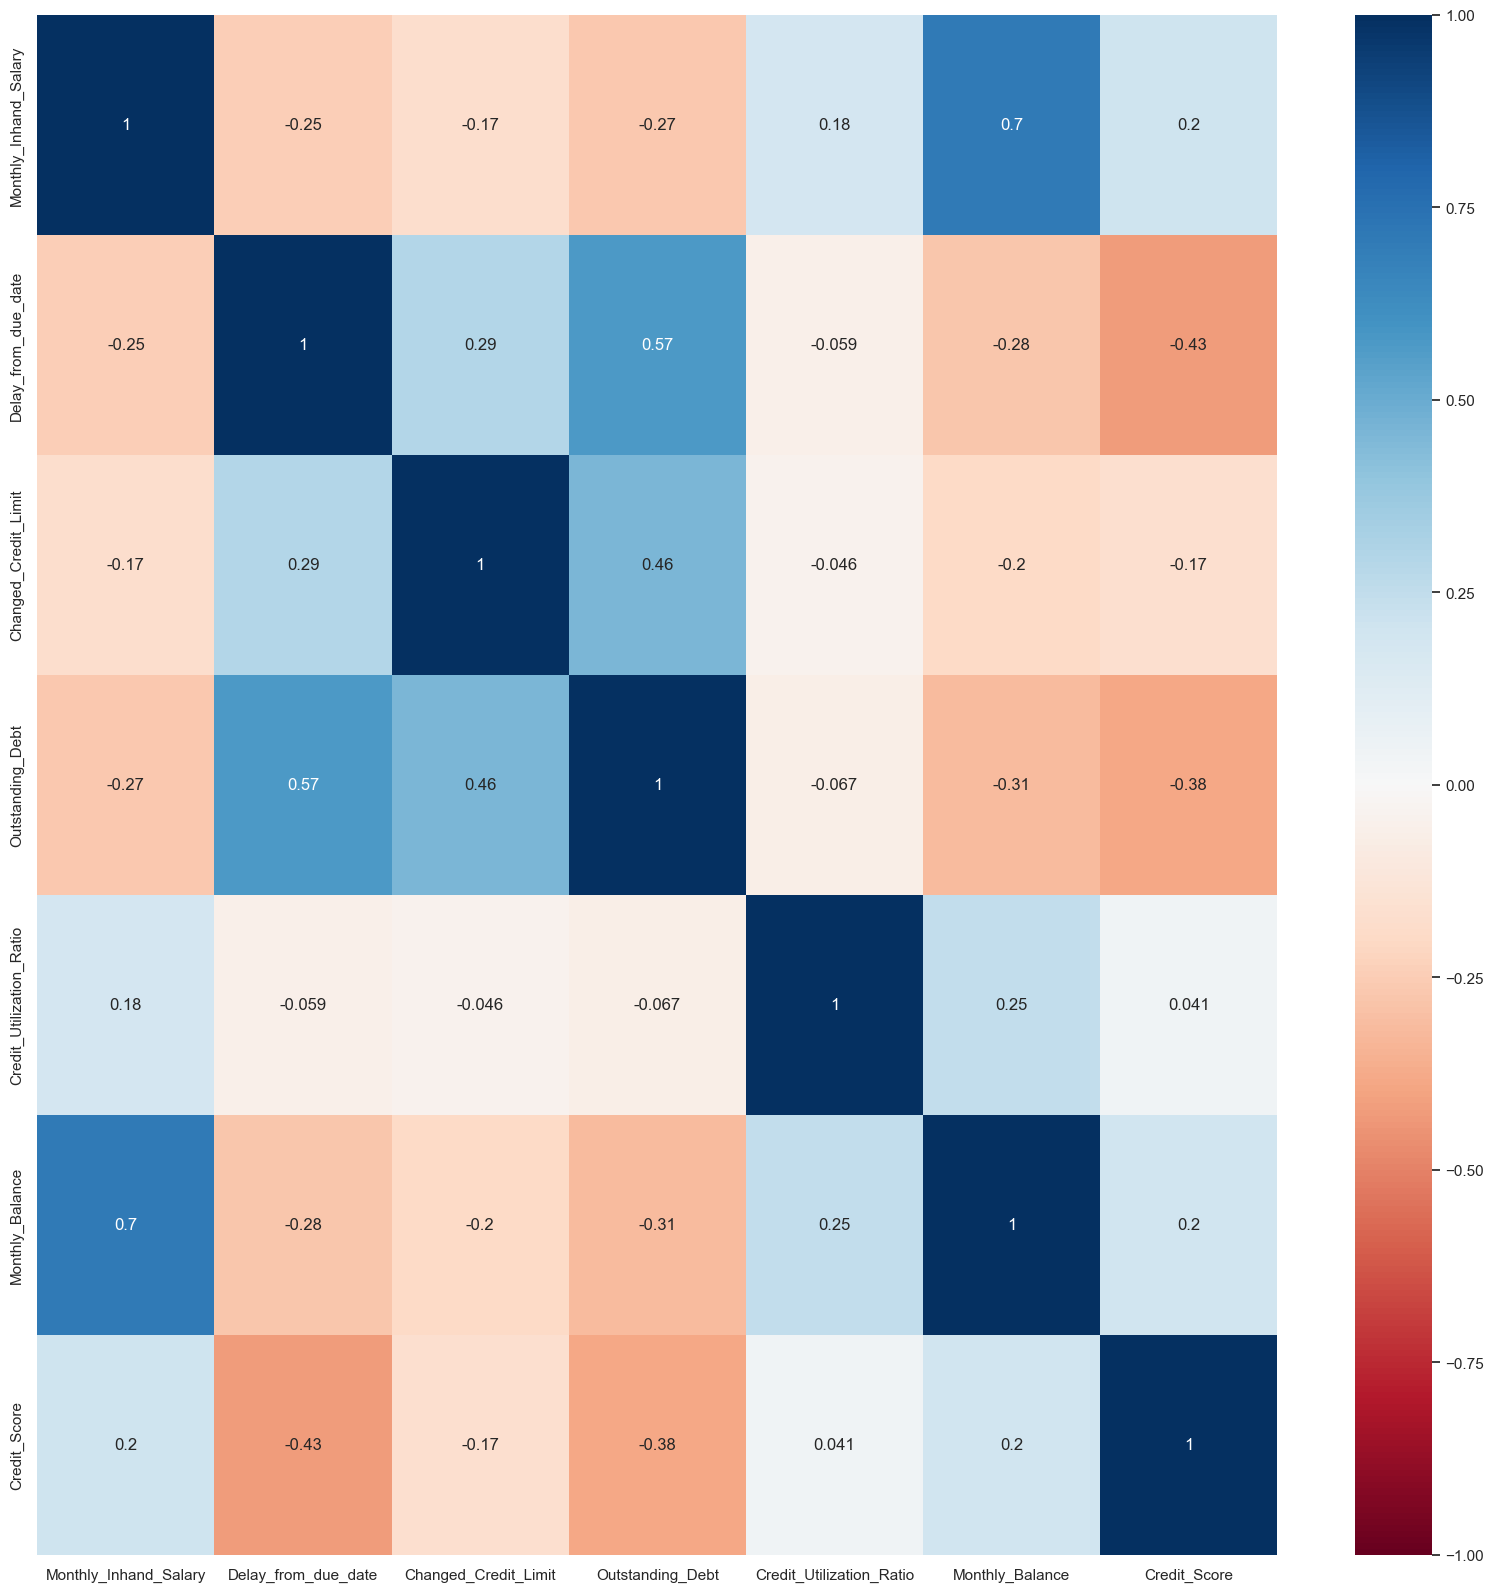
\includegraphics[width=\columnwidth]{images/credscoreheatmap.png}
    \caption{Heat map correlation.}
    \label{fig:figure1}
    \end{center}
\end{figure}
\section{Proposed methodology}
From the literature review and the fact that this problem involves multiclassification,
we decided to make and compare two SVM models with a linear and RBF kernel and one 
multinomial logistic regression model. We trained the logistic regression model with and without
outliters to determine the impact on the accuracy. For all three of our models, we used
the standard 80:20 training to testing split in order to benchmark the performance on unseen
data. Additionally, we used Streamlit to host our model online.

\section{Experimental results}
The Python library scikit-learn was used to create all four models. Both SVM models preserve default values aside from the change
in kernel type. The two multinomial logistic regression models also preserve default values aside from setting the maximum iterations
to two thousand, specifying the multi\_class parameter to ``multinomial'' and using the limited-memory BFGS solver.
For all models, the ``Standard'' credit score was most likely to be categorized correctly, followed by ``Poor'' and ``Good''. 
However, all models have relatively low accuracy overall. The SVM with a RBF kernel performed the best with an
accuracy of 0.62 (Figure 2). \vspace{5mm}\newline
In an attempt to improve the accuracy of the logistic regression model, which was performing the poorest, we removed outliers within the dataset.
This had very little impact on the overall accuracy, but the f1-score for the ``Good'' credit score improved the most, going from 0.22 to 0.37 (Figure 5).
Interestingly, the SVM model with a linear kernel was unable to classify a ``Good'' score at all, with zeroes for precision, 
recall, and f1-score (Figure 3). All models had a tendency to misclassify the ``Standard'' category the most as either ``Poor'' or 
``Good'' at similar frequency.\vspace{5mm}\newline
Since our data was imbalanced, we tested if a combination of oversampling and removing outliers can improve the accuracy of our SVM models. 
The result was that changes in accuracy were minimal. The SVM with a RBF kernel achieved a slightly lower accuracy while the SVM with a linear kernel
achieved a slightly higher accuracy. Oversampling, however, allowed both SVM models to achieve greater precision, recall,
and f1-scores.
\section{Project Roadmap}
Our problem from a scientifc standpoint
involves creating a reliable and predic-
tive model for assessing the creditworthi-
ness of individuals. This model has to
be created with various amounts of in-
put data and different features that goes
towards creditworthiness. This formula-
tion of credit score is complex and in-
volves constant refinement as new fea-
tures in the future can be used at input
data.
\vspace{5mm}\newline
To solve this problem, we must be edu-
cated on the problem first and that comes
with background studying and lots of re-
search on the topic of credit score. Our
group wants to finish this around the first
week after turning in the one-page write
up about our project. Since research is
very important in any project, we will
spend days to study up on the topic to
get the most information we can.
The next part of our project will con-
sist of dataset understanding and ex-
ploratory data analysis. In this part of
our project, we must spend time to un-
derstand our dataset fully to know how
to clean it up. The dataset is just as
important as the model as the dataset is
what helps the model learn to predict the
credit scores to solve our problem. We
will spend a total of 2 days or more af-
ter the background study to explore our
dataset. We will make many visualiza-
tions to understand our dataset.
After cleaning and understanding our
dataset, we will begin to build our ac-
curate prediction models. We estimate
around 1-2 weeks on this as developing
the models well will give use more accu-
rate predictions. We estimate a lot of
trial and error since we will be build-
ing multiple different models to find the
best model for our dataset. We will be
building a multinomial logistic regression
model, a SVM model with the linear ker-
nel, and a SVM model using the RBF
kernel.
\vspace{5mm}\newline
After building the models, we must eval-
uate each of them to find the best model.
Evaluating these models should take max
a week, because we will be focusing on
accuracy, precision, recall, and f1-score.
After a good evaluation of the models,
we will be picking the best one keeping in
mind also the constraints of our dataset.
The last thing we need to do is building
the basic web-based front-end to invoke
and run the model. Our group plans to
take the remaining amount of time we
have left to build the web-based front-
end and continue to test our model until
we believe there is nothing else we can
do.
\section*{Conclusion and discussion}
Of the three different models we trained, SVM model using the RBF Kernel yielded the highest
accuracy of 0.62. In our logistic model, removing the outliers caused a decrease in precison
and recall when predicting poor credit scores, but an increase when predicting standard and good
scores. Coincidentally, both logistic models ended up with an identical overall accuracy.
\vspace{5mm}\newline
The SVM model using the RBF kernel, had a noticibly higher precision when predicting poor credit
scores, meaning that a detected poor credit score is likely to be correct. This model also had a
very high recall for standard credit scores, meaning that it was able to correctly identify almost all
instances with a standard score.
\vspace{5mm}\newline
In all of our models, it was very difficult to correctly identify a high credit score. This could have
been caused by a much lower sample size when compared to entries of a poor or standard score. In particular,
the SVM using the linear kernel was unable to report precision, recall, and f1-score for high credit scores,
meaning that there was an insufficient amount of data correctly predict it. To fix some of these issues,
we could modify the training data to contain an equal number of good, standard, and poor credit score samples. 

\begin{thebibliography}{00}
\bibitem{b1} Dastile, X., Celik, T., \& Potsane, M. (2020).
Statistical and machine learning models in credit scoring: A systematic literature survey. Applied Soft Computing, 91. doi:10.1016/j.asoc.2020.106263.
\bibitem{b2} Dumitrescu, E., Hué, S., Hurlin, C., \& Tokpavi, S. (2022). 
Machine learning for credit scoring: Improving logistic regression 
with non-linear decision-tree effects. European Journal of Operational 
Research, 297(3), 1178-1192. doi:10.1016/j.ejor.2021.06.053
\end{thebibliography}

\begin{figure*}[h]
    % Below are the classification reports for each of the models:
    \begin{subtable}{0.5\textwidth}
        \centering
        \resizebox{\columnwidth}{!}{\begin{tabular}{|l|l|l|l|l|}
        \hline
            % RBF Kernel & ~ & ~ & ~ & ~ \\ \hline
            ~ & precision & recall & f1-score & support \\ \hline
            ~ & ~ & ~ & ~ & ~ \\ \hline
            Good & 0.59 & 0.06 & 0.1 & 2801 \\ \hline
        Poor & 0.66 & 0.57 & 0.61 & 4560 \\ \hline
        Standard & 0.6 & 0.83 & 0.7 & 8213 \\ \hline
        ~ & ~ & ~ & ~ & ~ \\ \hline
        accuracy & ~ & ~ & 0.62 & 15574 \\ \hline
        macro avg & 0.62 & 0.49 & 0.47 & 15574 \\ \hline
        weighted avg & 0.62 & 0.62 & 0.57 & 15574 \\ \hline
        \end{tabular}}
        \caption{Classification report for SVM with RBF kernel}
    \end{subtable}
    \begin{subfigure}{0.5\textwidth}
        \centering
        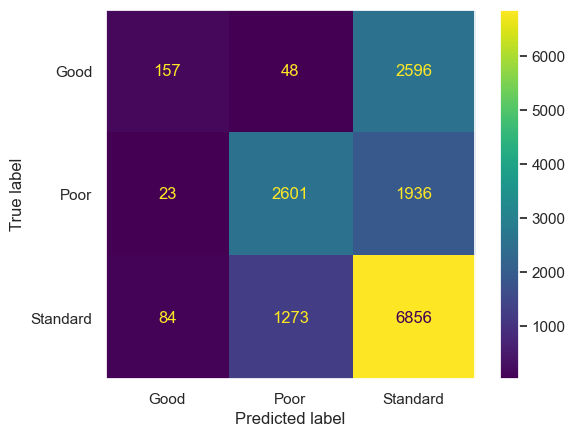
\includegraphics[width=0.65\columnwidth]{images/svmrbf.png}
        \caption{SVM, RBF kernel}
    \end{subfigure}
    \caption{SVM with RBF kernel and outliers}
\end{figure*}
\begin{figure*}[h]
    \begin{subtable}{0.5\textwidth}
        \centering
        \resizebox{\columnwidth}{!}{\begin{tabular}{|l|l|l|l|l|}
            \hline
            ~ & precision & recall & f1-score & support \\ \hline
            ~ & ~ & ~ & ~ & ~ \\ \hline
        Good & 0 & 0 & 0 & 2801 \\ \hline
        Poor & 0.59 & 0.44 & 0.5 & 4560 \\ \hline
        Standard & 0.56 & 0.84 & 0.68 & 8213 \\ \hline
        ~ & ~ & ~ & ~ & ~ \\ \hline
        accuracy & ~ & ~ & 0.57 & 15574 \\ \hline
        macro avg & 0.39 & 0.43 & 0.39 & 15574 \\ \hline
        weighted avg & 0.47 & 0.57 & 0.5 & 15574 \\ \hline
        \end{tabular}}
        \caption{Classification report for SVM with linear kernel}
    \end{subtable}
    \begin{subfigure}{0.5\textwidth}
        \centering
        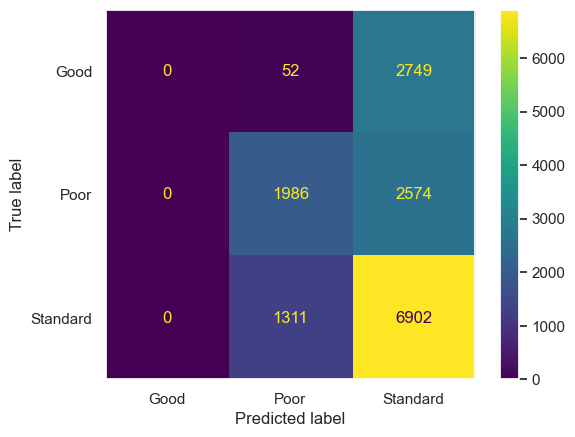
\includegraphics[width=0.65\columnwidth]{images/svmli.png}
        \caption{SVM, linear kernel}
    \end{subfigure}
    \caption{SVM with linear kernel and outliers}
\end{figure*}

\begin{figure*}[h]
    \begin{subtable}{0.5\textwidth}
        \centering
        \resizebox{\columnwidth}{!}{\begin{tabular}{|l|l|l|l|l|}
            \hline
            ~ & precision & recall & f1-score & support \\ \hline
            ~ & ~ & ~ & ~ & ~ \\ \hline
            Good & 0.4 & 0.75 & 0.52 & 2660 \\ \hline
        Poor & 0.62 & 0.68 & 0.65 & 3715 \\ \hline
        Standard & 0.75 & 0.49 & 0.59 & 7506 \\ \hline
        ~ & ~ & ~ & ~ & ~ \\ \hline
        accuracy & ~ & ~ & 0.59 & 13881 \\ \hline
        macro avg & 0.59 & 0.64 & 0.59 & 13881 \\ \hline
        weighted avg & 0.65 & 0.59 & 0.59 & 13881 \\ \hline
        \end{tabular}}
        \caption{}
    \end{subtable}
    \begin{subfigure}{0.5\textwidth}
        \centering
        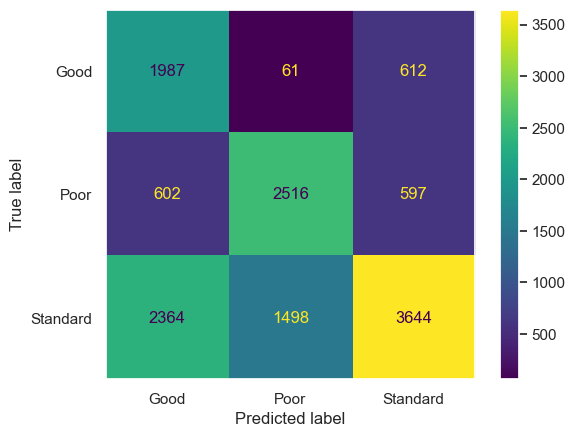
\includegraphics[width=0.65\columnwidth]{images/lioversample.png}
        \caption{}
    \end{subfigure}
    \caption{SVM linear w/ oversampling, no outliers}
\end{figure*}
\begin{figure*}[h]
    \begin{subtable}{0.5\textwidth}
        \centering
        \resizebox{\columnwidth}{!}{\begin{tabular}{|l|l|l|l|l|}
            \hline
            ~ & precision & recall & f1-score & support \\ \hline
            ~ & ~ & ~ & ~ & ~ \\ \hline
            Good & 0.41 & 0.75 & 0.53 & 2660 \\ \hline
        Poor & 0.63 & 0.7 & 0.66 & 3715 \\ \hline
        Standard & 0.76 & 0.5 & 0.6 & 7506 \\ \hline
        ~ & ~ & ~ & ~ & ~ \\ \hline
        accuracy & ~ & ~ & 0.6 & 13881 \\ \hline
        macro avg & 0.6 & 0.65 & 0.6 & 13881 \\ \hline
        weighted avg & 0.66 & 0.6 & 0.61 & 13881 \\ \hline
        \end{tabular}}
        \caption{}
    \end{subtable}
    \begin{subfigure}{0.5\textwidth}
        \centering
        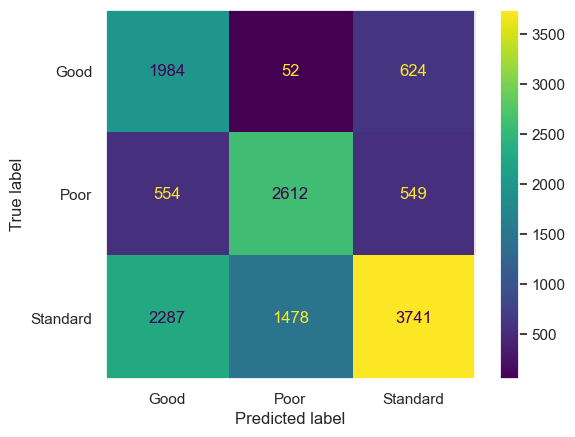
\includegraphics[width=0.65\columnwidth]{images/rbfoversample.png}
        \caption{}
    \end{subfigure}
    \caption{SVM RBF w/ oversampling, no outliers}
\end{figure*}
\begin{figure*}[h]
    \begin{subtable}{0.5\textwidth}
        \centering
        \resizebox{\columnwidth}{!}{\begin{tabular}{|l|l|l|l|l|}
        \hline
        ~ & precision & recall & f1-score & support \\ \hline
            ~ & ~ & ~ & ~ & ~ \\ \hline
            Good & 0.5 & 0.14 & 0.22 & 2801 \\ \hline
            Poor & 0.58 & 0.39 & 0.47 & 4560 \\ \hline
            Standard & 0.57 & 0.81 & 0.67 & 8213 \\ \hline
            ~ & ~ & ~ & ~ & ~ \\ \hline
            accuracy & ~ & ~ & 0.57 & 15574 \\ \hline
            macro avg & 0.55 & 0.45 & 0.45 & 15574 \\ \hline
            weighted avg & 0.56 & 0.57 & 0.53 & 15574 \\ \hline
        \end{tabular}}
        \caption{Classification report for logistic model with outliers}
    \end{subtable}
    \begin{subfigure}{0.5\textwidth}
        \centering
        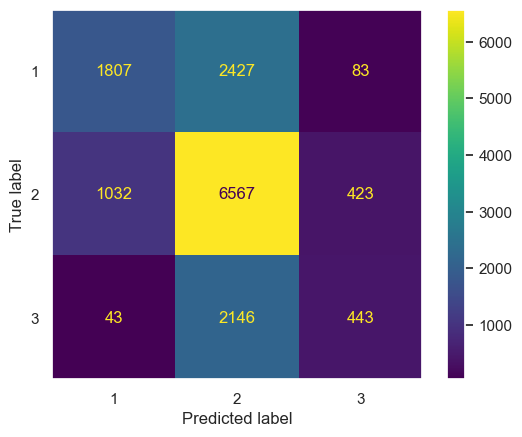
\includegraphics[width=0.65\columnwidth]{images/logisticWithOutliers.png}
        \caption{Logistic with outliers}
    \end{subfigure}
    \caption{}
\end{figure*}
\begin{figure*}[h]
    \begin{subtable}{0.5\textwidth}
        \centering
        \resizebox{\columnwidth}{!}{\begin{tabular}{|l|l|l|l|l|}
            \hline
            ~ & precision & recall & f1-score & support \\ \hline
            ~ & ~ & ~ & ~ & ~ \\ \hline
            Good & 0.52 & 0.28 & 0.37 & 2660 \\ \hline
            Poor & 0.62 & 0.4 & 0.49 & 3715 \\ \hline
            Standard & 0.61 & 0.81 & 0.69 & 7506 \\ \hline
            ~ & ~ & ~ & ~ & ~ \\ \hline
            accuracy & ~ & ~ & 0.6 & 13881 \\ \hline
            macro avg & 0.58 & 0.5 & 0.52 & 13881 \\ \hline
            weighted avg & 0.59 & 0.6 & 0.58 & 13881 \\ \hline
        \end{tabular}}
        \caption{Classification report for logistic model with no outliers}
    \end{subtable}
    \begin{subfigure}{0.5\textwidth}
        \centering
        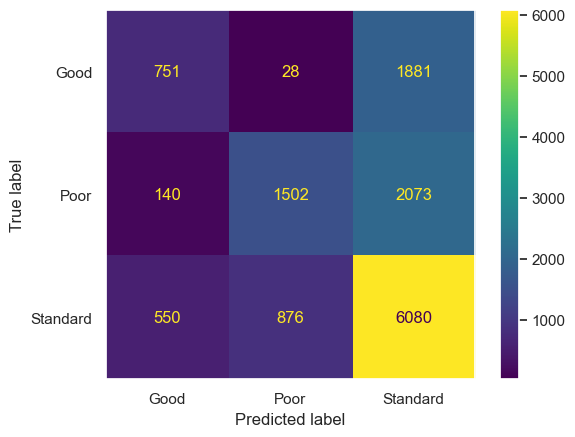
\includegraphics[width=0.65\columnwidth]{images/logisticNoOutliers.png}
        \caption{Logistic with no outliers}
    \end{subfigure}
    \caption{}
\end{figure*}


\end{document}
